\section{Tutorial Using Tetrahedral Mesh Created by LaGriT}
\label{sec:example:3dtet4}

PyLith features discussed in this tutorial:
\begin{itemize}
\item Quasi-static solution
\item LaGriT mesh format
\item Dirichlet boundary conditions
\item Kinematic fault interface conditions
\item Linearly elastic isotropic material
\item Maxwell linear viscoelastic material
\item Specifying more than one material
\item VTK output
\item Linear tetrahedral cells
\item SimpleDB spatial database
\item ZeroDispDB spatial database
\item Custom algebraic multigrid preconditioner with split fields
\item Global uniform mesh refinement
\end{itemize}
All of the files necessary to run the examples are contained in the
directory \filename{examples/3d/tet4.}


\subsection{Overview}

This tutorial is a simple 3D example of a quasi-static finite element
problem. It is a mesh composed of 852 linear tetrahedra subject to
displacement boundary conditions. This example demonstrates the usage
of the LaGriT mesh generation package \url{lagrit.lanl.gov} to create
a mesh, as well as describing how to use a LaGriT-generated mesh in
PyLith. In this tutorial, we will walk through the steps necessary
to construct, run, and visualize the results for two problems that
use the same mesh. For each of these problems we also consider a simulation
using a custom algebraic multigrid preconditioner with a globally
uniformly refined mesh that reduces the node spacing by a factor of
two. In addition to this manual, each of the files for the example
problems includes extensive comments.


\subsection{Mesh Generation and Description}

The mesh for these examples is a simple rectangular prism (Figure
\vref{fig:3dtet4:mesh}). This mesh would be quite difficult to generate
by hand, so we use the LaGriT mesh generation package. For this example,
we provide a documented command file in \filename{examples/3d/tet4.}
Examination of this command file should provide some insight into
how to use LaGriT with PyLith. For more detailed information refer
to the LaGriT website \url{lagrit.lanl.gov}. If you have LaGriT installed
on your machine, you can use the command file to create your own mesh.
Otherwise, you can use the mesh that has already been created.

There are two ways to use the command file. The simplest method is
to go to the \filename{examples/3d/tet4} directory, start LaGriT, and then type:
\begin{shell}
input mesh_tet4_1000m.lagrit
\end{shell}
This will run the commands in that file, which will produce the necessary
files to run the example. This method will create the mesh, but you
will gain very little insight into what is being done. A more informative
approach is to input each command directly. That way, you will see
what each command does. You can simply copy and paste the commands
from \filename{mesh\_tet4\_1000m.lagrit}. For example, the first six
commands, which define the block shape, are
\begin{shell}
define / domain_xm / -3.0e+3
define / domain_xp /  3.0e+3
define / domain_ym / -3.0e+3
define / domain_yp /  3.0e+3
define / domain_zm / -4.0e+3
define / domain_zp /  0.0e+3 
\end{shell}
Continuing through the remainder of the commands in \filename{mesh\_tet4\_1000m.lagrit},
you will eventually end up with the files \filename{tet4\_1000m\_binary.gmv},
\filename{tet4\_1000m\_ascii.gmv}, \filename{tet4\_1000m\_ascii.pset},
and \filename{tet4\_1000m\_binary.pset}. The ASCII files are not actually
needed, but we create them so users can see what is contained in the
files. These files may also be used instead of the binary versions,
if desired. The \filename{.gmv} files define the mesh information, and
they may be read directly by the GMV \url{laws.lanl.gov/XCM/gmv/GMVHome.html}
mesh visualization package. The \filename{.pset} files specify the vertices
corresponding to each set of vertices on a surface used in the problem,
including the fault as well as external boundaries to which boundary
conditions are applied.

\begin{figure}
  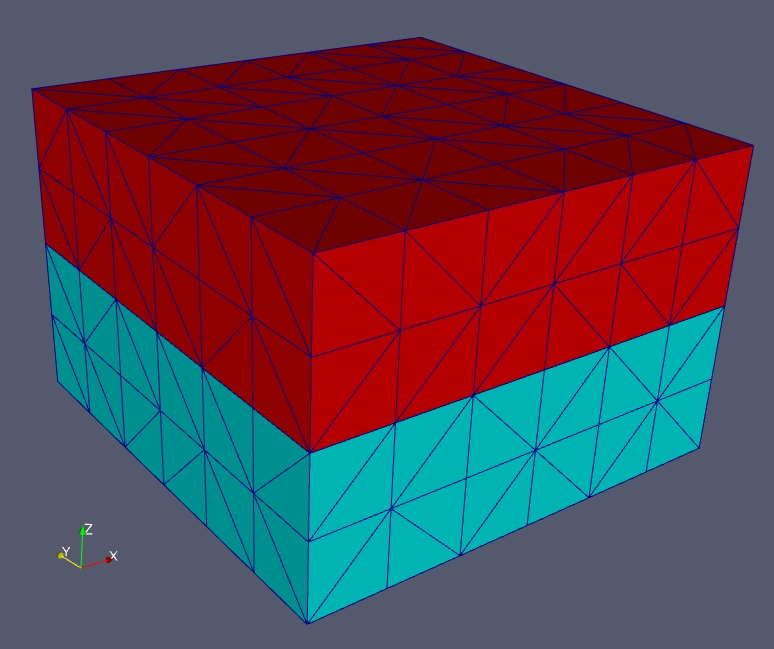
\includegraphics[scale=0.45]{examples/figs/3dtet4_mesh}
  \caption{Mesh composed of linear tetrahedral cells generated by
    LaGriT used for the example problems. The different colors
    represent the different materials.}
  \label{fig:3dtet4:mesh}
\end{figure}


\subsection{Additional Common Information}

In addition to the mesh, the example problems share additional information.
In such cases it is generally useful to create a file named \filename{pylithapp.cfg}
in the run directory, since this file is read automatically every
time PyLith is run. Settings specific to a particular problem may
be placed in other \filename{.cfg} files, as described later, and then
those files are placed on the command line.  The settings contained
in \filename{pylithapp.cfg} for this problem consist of:
\begin{inventory}
  \facilityitem{pylithapp.journal.info}{Settings that control the verbosity of
    the output for the different components.}
  \facilityitem{pylithapp.mesh\_generator}{Settings that control mesh importing,
    such as the importer type, the filenames, and the spatial dimension
    of the mesh.}
  \facilityitem{pylithapp.timedependent}{Settings that control the problem, such
    as the total time, time-step size, and number of entries in the material
    array.}
  \facilityitem{pylithapp.timedependent.materials}{Settings that control the material
    type, specify which material IDs are to be associated with a particular
    material type, and give the name of the spatial database containing
    material parameters for the mesh. The quadrature information is also
    given.}
  \facilityitem{pylithapp.petsc}{PETSc settings to use for the problem, such as
    the preconditioner type.}
\end{inventory}
Since these examples use a mesh from LaGriT, we set the importer to
\object{MeshIOLagrit}:
\begin{cfg}
<h>[pylithapp.mesh_generator]</h>
<f>reader</f> = pylith.meshio.MeshIOLagrit

<h>[pylithapp.mesh_generator.reader]</h>
<p>filename_gmv</p> = mesh/tet4_1000m_binary.gmv
<p>filename_pset</p> = mesh/tet4_1000m_binary.pset
<p>flip_endian</p> = True
# record_header_32bit = False
\end{cfg}
Notice that there are a couple of settings pertinent to binary files.
The first flag (\texttt{flip\_endian}) is used if the binary files
were produced on a machine with a different endianness than the machine
on which they are being read. If you get an error when attempting
to run an example, you may need to change the setting of this flag.
The second flag (\texttt{record\_header\_32bit}) may need to be set
to \texttt{False} if the version of LaGriT being used has 64-bit Fortran
record headers. 

This example differs from previous examples, because we specify two
material groups:
\begin{cfg}
<h>[pylithapp.timedependent]</h>
<f>materials</f> = [elastic, viscoelastic]

<h>[pylithapp.timedependent.materials.elastic]</h>
<p>label</p> = Elastic material
<p>id</p> = 1
<p>db.iohandler.filename</p> = spatialdb/mat_elastic.spatialdb
<f>quadrature.cell</f> = pylith.feassemble.FIATSimplex
<p>quadrature.cell.dimension</p> = 3

<h>[pylithapp.timedependent.materials.viscoelastic]</h>
<p>label</p> = Viscoelastic material
<p>id</p> = 2
<p>db.iohandler.filename</p> = spatialdb/mat_viscoelastic.spatialdb
<f>quadrature.cell</f> = pylith.feassemble.FIATSimplex
<p>quadrature.cell.dimension</p> = 3
\end{cfg}
The two materials correspond to the two different colors in Figure
\vref{fig:3dtet4:mesh}. Each material uses a different spatial database
because the physical parameters are different. In generating the mesh
within LaGriT, the mesh contains four materials as a result of how
LaGriT handles materials and interior interfaces. Near the end of
the LaGriT command file, we merge the materials on each side of the
fault into a single material to simplify the input and output from
PyLith. For this example, values describing three-dimensional elastic
material properties are given by the single point in the spatial databases,
resulting in uniform physical properties within each material.


\subsection{Shear Displacement Example}

The first example problem is shearing of the mesh along the y-direction,
with displacement boundary conditions applied on the planes corresponding
to the minimum and maximum x-values. Parameter settings that override
or augment those in \filename{pylithapp.cfg} are contained in the file
\filename{step01.cfg}. These settings are:
\begin{inventory}
  \facilityitem{pylithapp.timedependent}{Specifies an implicit formulation for
    the problem and specifies the array of boundary conditions.}
  \facilityitem{pylithapp.timedependent.implicit}{Specifies an array of two output
    managers, one for the full domain, and another for a subdomain corresponding
    to the ground surface.}
  \facilityitem{pylithapp.timedependent.bc.x\_pos}{Specifies the boundary conditions
    for the right side of the mesh, defining which degrees of freedom
    are being constrained (\texttt{x} and \texttt{y}), providing the label
    (defined in \filename{tet4\_1000m\_binary.pset}) defining the points
    desired, assigning a label to the boundary condition set, and giving
    the name of the spatial database defining the boundary conditions
    (\filename{fixeddisp\_shear.spatialdb}).}
  \facilityitem{pylithapp.timedependent.bc.x\_neg}{Specifies the boundary conditions
    for the left side of the mesh, defining which degrees of freedom are
    being constrained (\texttt{x} and \texttt{y}), providing the label
    (defined in \filename{tet4\_1000m\_binary.}pset) defining the points
    desired, assigning a label to the boundary condition set, and giving
    the name of the spatial database defining the boundary conditions
    (\filename{fixeddisp\_shear.spatialdb}).}
  \facilityitem{pylithapp.timedependent.bc.z\_neg}{Specifies the boundary conditions
    for the bottom of the mesh, defining which degrees of freedom are
    being constrained (\texttt{x} and \texttt{y}), providing the label
    (defined in \filename{tet4\_1000m\_binary.}pset) defining the points
    desired, assigning a label to the boundary condition set, and giving
    the name of the spatial database defining the boundary conditions
    (\filename{fixeddisp\_shear.spatialdb}).}
  \facilityitem{pylithapp.problem.formulation.output.domain.writer}{Gives the
    base filename for VTK output over the entire domain (\filename{shearxy.vtk}).}
  \facilityitem{pylithapp.problem.formulation.output.subdomain}{Gives the label
    of the nodeset defining the subdomain and gives the base filename
    for VTK output over the subdomain corresponding to the ground surface
    (\filename{step01-groundsurf.vtk}).}
  \facilityitem{pylithapp.timedependent.materials.elastic.output}{Gives the base
    filename for state variable output files for the \texttt{elastic}
    material set (\filename{step01-elastic.vtk}), and causes state variables
    to be averaged over all quadrature points in each cell.}
  \facilityitem{pylithapp.timedependent.materials.viscoelastic.output}{Gives the
    base filename for state variable output files for the \texttt{viscoelastic}
    material set (\filename{step01-viscoelastic.vtk}), and causes state
    variables to be averaged over all quadrature points in each cell.}
\end{inventory}
The values for the Dirichlet boundary conditions are described in
the file \filename{fixeddisp\_shear.spatialdb}, as specified in \filename{step01.cfg}.
The format of all spatial database files is similar. Because data
are being specified using two control points (rather than being uniform
over the mesh, for example), the data dimension is one.

The files containing common information
(\filename{tet4\_1000m\_binary.gmv},
\filename{tet4\_1000m\_binary.pset}, \filename{pylithapp.cfg},
\filename{mat\_elastic.spatialdb}, and
\filename{mat\_viscoelastic.spatialdb}) along with the
problem-specific files (\filename{step01.cfg} and
\filename{fixeddisp\_shear.spatialdb}) provide a complete description
of the problem, and we can then run this example by typing
\begin{shell}
$$ pylith step01.cfg
\end{shell}
Once the problem has run, six files will be produced. The first file
is named \filename{step01\_t0000000.vtk}. The \filename{t0000000}
indicates that the output is for the first (and only) time step,
corresponding to an elastic solution. This file contains mesh
information as well as displacement values at the mesh vertices. The
second file is named
\filename{step01-statevars-elastic\_t0000000.vtk}. This file contains
the state variables for each cell in the material group
\texttt{elastic}.  The default fields are the total strain and stress
fields. These values are computed at each quadrature point in the
cell. We have requested that the values be averaged over all
quadrature points for each cell; however, since we only have a single
quadrature point for each linear tetrahedron, this will have no
effect. The third file
(\filename{step01-statevars-viscoelastic\_info.vtk}) gives the
material properties used for the \texttt{viscoelastic} material
set. Since we have not specified which properties to write, the
default properties (\texttt{mu}, \texttt{lambda}, \texttt{density})
are written.  There are two additional files containing the state
variables for each of the material sets. The final file
(\filename{step01-groundsurf\_t0000000.vtk}) is analogous to
\filename{step01\_t0000000.vtk}, but in this case the results are only
given for a subset of the mesh corresponding to the ground
surface. Also, the cells in this file are one dimension lower than the
cells described in \filename{step01\_t0000000.vtk}, so they are
triangles rather than tetrahedra. All of the \filename{.vtk} files may
be used with a number of visualization packages. If the problem ran
correctly, you should be able to generate a figure such as Figure
\vref{fig:3dtet4:shear}, which was generated using ParaView.

\begin{figure}
  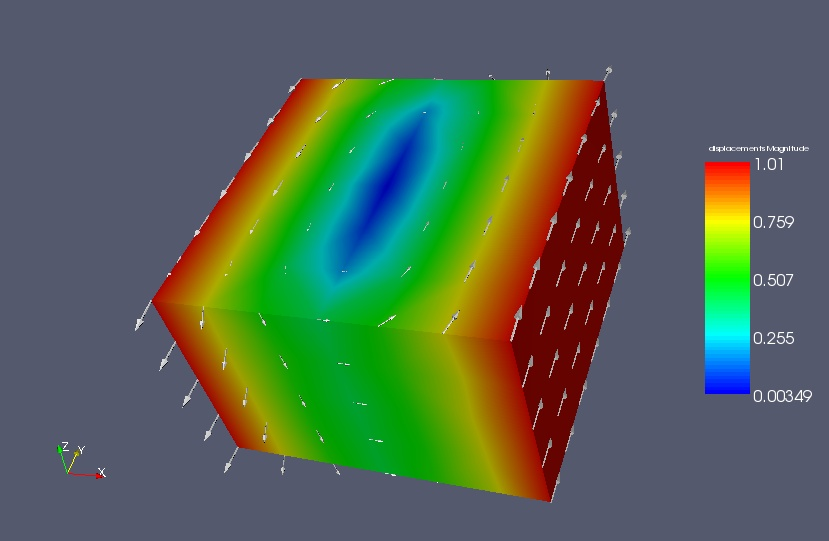
\includegraphics[scale=0.45]{examples/figs/3dtet4_shear}
  \caption{Color contours and vectors of displacement for the axial displacement
    example using a mesh composed of linear tetrahedral cells generated
    by LaGriT.}
  \label{fig:3dtet4:shear}
\end{figure}


\subsubsection{Alternative Solver and Discretization Settings}

Example \filename{step01.cfg} uses the additive Schwarz preconditioner
in conjunction with a classical Gram-Schmidt orthogonalization iterative
solver. This preconditioner works reasonably well but the number of
iterations generally scales with problem size. Even this small, simple
problem requires 24 iterations. In this example (\filename{step02.cfg}),
we use a more sophisticated preconditioner that preconditions the
degrees of freedom associated with the displacement field with an
algebraic multigrid algorithm (see Section \vref{sec:petsc:options}
for details). Additionally, we illustrate the use of global uniform
mesh refinement to increase the resolution of the solution by a factor
of two. Because the mesh is refined in parallel after distribution,
this technique can be used to run a larger problem than would be possible
if the full resolution mesh had to be generated by the mesh generator.
LaGriT runs only in serial and CUBIT has extremely limited parallel
mesh generation capabilities. Table \vref{tab:3dtet4:solver:cmp} shows
the improved efficiency of the solver using the split fields with
the algebraic multigrid preconditioner, especially as the problem
size becomes larger. We have found similar results for other problems.

\begin{table}[htbp]
  \caption{Number of iterations in linear solve for the Shear
    Displacement and Kinematic Fault Slip problems discussed in this
    section. The preconditioner using split fields and an algebraic
    multigrid algorithm solves the linear system with fewer iterations
    with only a small to moderate increase as the problem size grows.}
\label{tab:3dtet4:solver:cmp}
\begin{tabular}{lp{2.0in}ccc}
\textbf{Problem} & \textbf{Preconditioner} & \textbf{Refinement} & \textbf{\# DOF} & \textbf{\# Solve Iterations}\\
\hline 
Shear Displacement & additive Schwarz & none & 546 & 24 (step01) \\
 &  & 2x  & 3890 & 47 \\
 & split fields with algebraic multigrid & none & 546 & 13 \\
 &  & 2x  & 3890 & 28 (step02)\\
Kinematic Fault Slip & additive Schwarz & none & 735 & 28 (step03) \\
 &  & 2x  & 4527 & 63\\
 & split fields with algebraic multigrid & none & 735 & 28 \\
 &  & 2x  & 4527 & 38 (step04) \\
\hline 
\end{tabular}
\end{table}

The field splitting and algebraic multigrid preconditioning are set
up in \filename{step02.cfg} with the following parameters:
\begin{cfg}
<h>[pylithapp.timedependent.formulation]</h>
<p>matrix_type</p> = aij

<h>[pylithapp.petsc]</h>
<p>pc_type</p> = ml
\end{cfg}
The uniform global refinement requires changing just a single parameter:
\begin{cfg}
<h>[pylithapp.mesh_generator]</h>
<f>refiner</f> = pylith.topology.RefineUniform
\end{cfg}

\subsection{Kinematic Fault Slip Example}

The next example problem is a right-lateral fault slip applied on
the vertical fault defined by \texttt{x = 0}. The left and right sides
of the mesh are fixed in the \texttt{x}, \texttt{y}, and \texttt{z}
directions. Parameter settings that override or augment those in \filename{pylithapp.cfg}
are contained in the file \filename{step03.cfg}. These settings are:
\begin{inventory}
  \facilityitem{pylithapp.timedependent}{Specifies an implicit formulation for
    the problem, the array of boundary conditions, and the array of interfaces.}
  \facilityitem{pylithapp.timedependent.implicit}{Specifies an array of two output
    managers, one for the full domain, and another for a subdomain corresponding
    to the ground surface.}
  \facilityitem{pylithapp.timedependent.bc.x\_pos}{Specifies the boundary conditions
    for the right side of the mesh, defining which degrees of freedom
    are being constrained (\texttt{x}, \texttt{y}, and \texttt{z}), providing
    the label (defined in \filename{tet4\_1000m\_binary.pset}) defining
    the points desired, and assigning a label to the boundary condition
    set. Rather than specifying a spatial database file to define the
    boundary conditions, we use the default spatial database (ZeroDispDB)
    for the Dirichlet boundary condition, which sets the displacements
    to zero.}
  \facilityitem{pylithapp.timedependent.bc.x\_neg}{Specifies the boundary conditions
    for the left side of the mesh, defining which degrees of freedom are
    being constrained (\texttt{x}, \texttt{y}, and \texttt{z}), providing
    the label (defined in \filename{tet4\_1000m\_binary.pset}) defining
    the points desired, and assigning a label to the boundary condition
    set. Rather than specifying a spatial database file to define the
    boundary conditions, we use the default spatial database (ZeroDispDB)
    for the Dirichlet boundary condition, which sets the displacements
    to zero.}
  \facilityitem{pylithapp.timedependent.interfaces}{Gives the label (defined in
    \filename{tet4\_1000m\_binary.pset}) defining the points on the fault,
    provides quadrature information, and then gives database names for
    material properties (needed for conditioning), fault slip, peak fault
    slip rate, and fault slip time.}
  \facilityitem{pylithapp.problem.formulation.output.output.writer}{Gives the
    base filename for VTK output over the entire domain (\filename{step03.vtk}).}
  \facilityitem{pylithapp.problem.formulation.output.subdomain}{Gives the label
    of the nodeset defining the subdomain and gives the base filename
    for VTK output over the subdomain corresponding to the ground surface
    (\filename{step03-groundsurf.vtk}).}
  \facilityitem{pylithapp.timedependent.interfaces.fault.output.writer}{Gives
    the base filename for cohesive cell output files 
    (\filename{step03-fault.vtk}).}
  \facilityitem{pylithapp.timedependent.materials.elastic.output}{Gives the base
    filename for state variable output files for the \texttt{elastic}
    material set (\filename{step03-statevars-elastic.vtk}), and causes state
    variables to be averaged over all quadrature points in each cell.}
  \facilityitem{pylithapp.timedependent.materials.viscoelastic.output}{Gives the
    base filename for state variable output files for the \texttt{viscoelastic}
    material set (\filename{step03-statevars-viscoelastic.vtk}), and causes
    state variables to be averaged over all quadrature points in each
    cell.}
\end{inventory}
The fault example requires three additional database files that were
not needed for the simple displacement example. The first file
(\filename{finalslip.spatialdb}) specifies a constant value of 2 m of
right-lateral fault slip that then tapers linearly to zero from 2 km
to 4 km depth, and a linearly-varying amount of reverse slip, with a
maximum of 0.25 m at the surface, linearly tapering to 0 m at 2 km
depth. The data dimension is one since the data vary linearly along a
vertical line. The default slip time function is a step-function, so
we also must provide the time at which slip begins. The elastic
solution is associated with advancing from $t=-dt$ to $t=0$, so we set
the slip initiation time for the step-function to 0 in
\filename{dislocation\_sliptime.spatialdb}.

The files containing common information
(\filename{tet4\_1000m\_binary.gmv},
\filename{tet4\_1000m\_binary.pset}, \filename{pylithapp.cfg},
\filename{mat\_elastic.spatialdb}, and
\filename{mat\_viscoelastic.spatialdb}) along with the
problem-specific files (\filename{step03.cfg},
\filename{finalslip.spatialdb}, and \filename{sliptime.spatialdb})
provide a complete description of the problem, and we can then run
this example by typing
\begin{shell}
$$ pylith step03.cfg
\end{shell}
Once the problem has run, eight files will be produced. The first file
is named \filename{step03\_t0000000.vtk}. The \filename{t0000000}
indicates that the output is for the first (and only) time step,
corresponding to an elastic solution. This file contains mesh
information as well as displacement values at the mesh vertices. The
second file is named
\filename{step03-statevars-elastic\_t0000000.vtk}. This file contains
the state variables for each cell in the material group
\texttt{elastic}.  The default fields are the total strain and stress
fields. We have requested that the values be averaged over all
quadrature points for each cell; however, since we only have a single
quadrature point for each linear tetrahedron, this will have no
effect. The third file
(\filename{step03-statevars-viscoelastic\_info.vtk}) gives the
material properties used for the \texttt{viscoelastic} material
set. Since we have not specified which properties to write, the
default properties (\texttt{mu}, \texttt{lambda}, \texttt{density})
are written. There are two additional files containing the state
variables for each of the material sets. The file
\filename{step03-groundsurf\_t0000000.vtk} is analogous to
\filename{step03\_t0000000.vtk}, but in this case the results are only
given for a subset of the mesh corresponding to the ground
surface. Also, the cells in this file are one dimension lower than the
cells described in \filename{step03\_t0000000.vtk}, so they are
triangles rather than tetrahedra. The file
\filename{step03-fault\_t0000000.vtk} gives the specified fault slip
for each vertex on the fault, along with the computed traction change
for the cohesive cell. The final file,
\filename{step03-fault\_info.vtk}, provides information such as the
normal direction, final slip, and slip time for each vertex on the
fault. All of the \filename{.vtk} files may be used with a number of
visualization packages. If the problem ran correctly, you should be
able to generate a figure such as Figure\vref{fig:3dtet:dislocation},
which was generated using ParaView.

\begin{figure}
  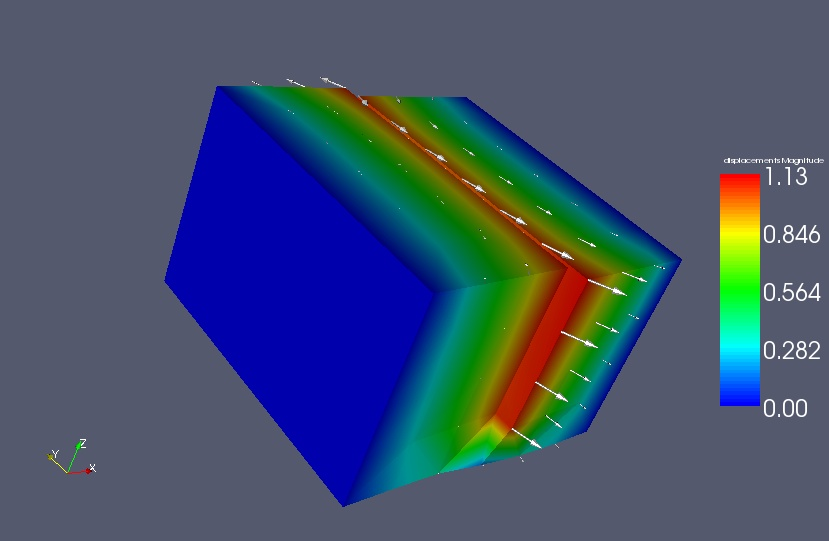
\includegraphics[scale=0.45]{examples/figs/3dtet4_dislocation}
  \caption{Color contours and vectors of displacement for the
    kinematic fault example using a mesh composed of linear
    tetrahedral cells generated by LaGriT.}
  \label{fig:3dtet:dislocation}
\end{figure}


\subsubsection{Alternative Solver and Discretization Settings}

As we did for the Shear Dislocation examples, in \filename{step04.cfg}
we switch to using the split fields and algebraic multigrid preconditioner
along with global uniform mesh refinement. Because PyLith implements
fault slip using Lagrange multipliers, we make a few small adjusments
to the solver settings. As discussed in Section \vref{sec:petsc:options},
we use a custom preconditioner for the Lagrange multiplier degrees
of freedom when preconditioning with field splitting. Within \filename{step04.cfg}
we turn on the use of the custom preconditioner for the Lagrange multiplier
degrees of freedom and add the corresponding settings for the fourth
field for the algebraic multigrid algorithm,
\begin{cfg}
<h>[pylithapp.timedependent.formulation]</h>
<p>split_fields</p> = True
<p>use_custom_constraint_pc</p> = True
<p>matrix_type</p> = aij

<h>[pylithapp.petsc]</h>
<p>fs_pc_type</p> = fieldsplit
<p>fs_pc_use_amat</p> = true
<p>fs_pc_fieldsplit_type</p> = multiplicative
<p>fs_fieldsplit_displacement_pc_type</p> = ml
<p>fs_fieldsplit_lagrange_multiplier_pc_type</p> = jacobi
<p>fs_fieldsplit_displacement_ksp_type</p> = preonly
<p>fs_fieldsplit_lagrange_multiplier_ksp_type</p> = preonly
\end{cfg}
Table \vref{tab:3dtet4:solver:cmp} shows the improved efficiency of
the solver using the split fields with the algebraic multigrid preconditioner.


% End of file
